\chapter{Resultados}

Para analisar o tempo de execução real das duas implementações é preciso primeiramente verificar se os resultados obtidos são corretos, e posteriormente verificar o quão grande foi a redução do tempo de execução comparado a versão sequencial dos algoritmos. Nesse capítulo serão estudados esses dois fatores.

\section{Autenticação dos resultados}

Algo imprescindível em algoritmos de processamento e análise de dados para que possam ser efetivamente usados em pesquisas é a confiabilidade dos resultados obtidos. Nem sempre é possível, apenas observando os resultados, saber se os mesmos estão certos ou errados. Portanto é preciso ter total confiança de que os dados obtidos da execução do algoritmo estão corretos.

Por esse motivo, o pequeno número de alterações feitas no código é tão importante, pois evita que erros sejam cometidos no processo de conversão. Além disso, em todos os testes realizados, os resultados obtidos das implementações em OpenMP e CUDA foram comparados com os do sequencial, e em todos os casos os mesmos foram idênticos, comprovando que os resultados estão corretos.

\section{Avaliação do tempo de execução}

Contudo, a principal motivação da implementação paralela desses algoritmos é a redução do tempo de execução. Para comparar o desempenho das implementações em OpenMP e CUDA com a implementação sequencial foram realizados diversos testes, com diferentes parâmetros, e em diferentes configurações de Hardware, com o intuito de medir o tempo real de execução dos mesmos para então verificar se houve uma redução significativa desse tempo.

Nos testes da implementação em OpenMP foram utilizados os seguintes processadores:

\begin{table}[H]
\caption{Modelos CPU}
\begin{center}
\begin{tabular}{cccc}
 & \textbf{AMD Opteron} & \textbf{Intel I5} & \textbf{Intel I7} \\
\hline\hline
\textbf{Clock}				& 2.8 GHz	& 3.3 Ghz	& 3.0 Ghz \\
\textbf{Total de núcleos}	& 8			& 4			& 8
\end{tabular} 
\end{center}
\end{table}

Já nos testes da implementação em CUDA foram utilizados as seguintes placas-de-vídeo:

\begin{table}[H]
\caption{Modelos GPU}
\begin{center}
\begin{tabular}{ccccc}
 & \textbf{9600GT} & \textbf{GTX480} & \textbf{Tesla C1060} & \textbf{Tesla C2050}\\
\hline\hline
\textbf{Clock}				& 1.96 GHz	& 1.4 GHz 	& 1.3 GHz	& 1.15 GHz \\
\textbf{Total de Memória}		& 512 MB		& 1536 MB	& 4096 MB	& 2687 MB \\
\textbf{Clock da Memória}	& 900 Mhz	& 1848 Mhz 	& 800 Mhz	& 1500 Mhz \\
\textbf{Núcleos CUDA}		& 64			& 480		& 240		& 448 \\
\textbf{Threads por bloco}	& 512		& 1024		& 512		& 1024
\end{tabular} 
\end{center}
\end{table}

Além disso, na versão CUDA foi utilizado como parâmetro de execução 16 threads por bloco. O número total de blocos e ciclos foram calculados diretamente pelo programa em relação ao tamanho do dado de entrada. Sendo assim, é perceptível que não foi feita nenhuma calibração mais otimizada. Tal decisão foi feita propositalmente em vista que tais ajustes podem variar de uma máquina para outra ou até mesmo de uma entrada para outra, e assumindo que tais programas deverão ser executados por pesquisadores e que os mesmos não teriam tempo e/ou conhecimento para fazer tais ajustes.

Os tempos foram marcados utilizando o comando \texttt{time} do Linux, e portanto são referentes a execução completa do programa, e não só apenas da execução do algoritmo de processamento em si.

\subsection{Resultados obtidos com o algoritmo Filtro de Lanczos}

Nos testes do algoritmo Filtro de Lanczos foi usado como dado de entrada uma matriz de 144 por 73 que contém as informações da temperatura diária de todo o globo entre 1950 e 2011, totalizando aproximadamente 22000 valores para cada quadrícula. Desse total, foram usados entre 5000 e 21000 valores nos testes realizados.

Nas duas implementações houve uma grande redução do tempo de execução em relação ao tempo da execução sequencial do mesmo, como demonstrado nas figuras \ref{fig:graficos_lanczos_cuda} e \ref{fig:graficos_lanczos_omp}. O melhor resultado foi obtido na execução da implementação em CUDA na GPU GTX480, a qual obteve uma melhora de trinta vezes em relação a execução sequencial numa CPU Intel I7. Com a implementação em OpenMP se obteve uma redução de apenas três vezes.

%%%%%%%%%%%%%%%%%%%%%%%%%%%%%%%%%%%%%%%%%%%%%%%%%%%%%%%%%%
% FIGURA
\begin{figure}[H]
\centering
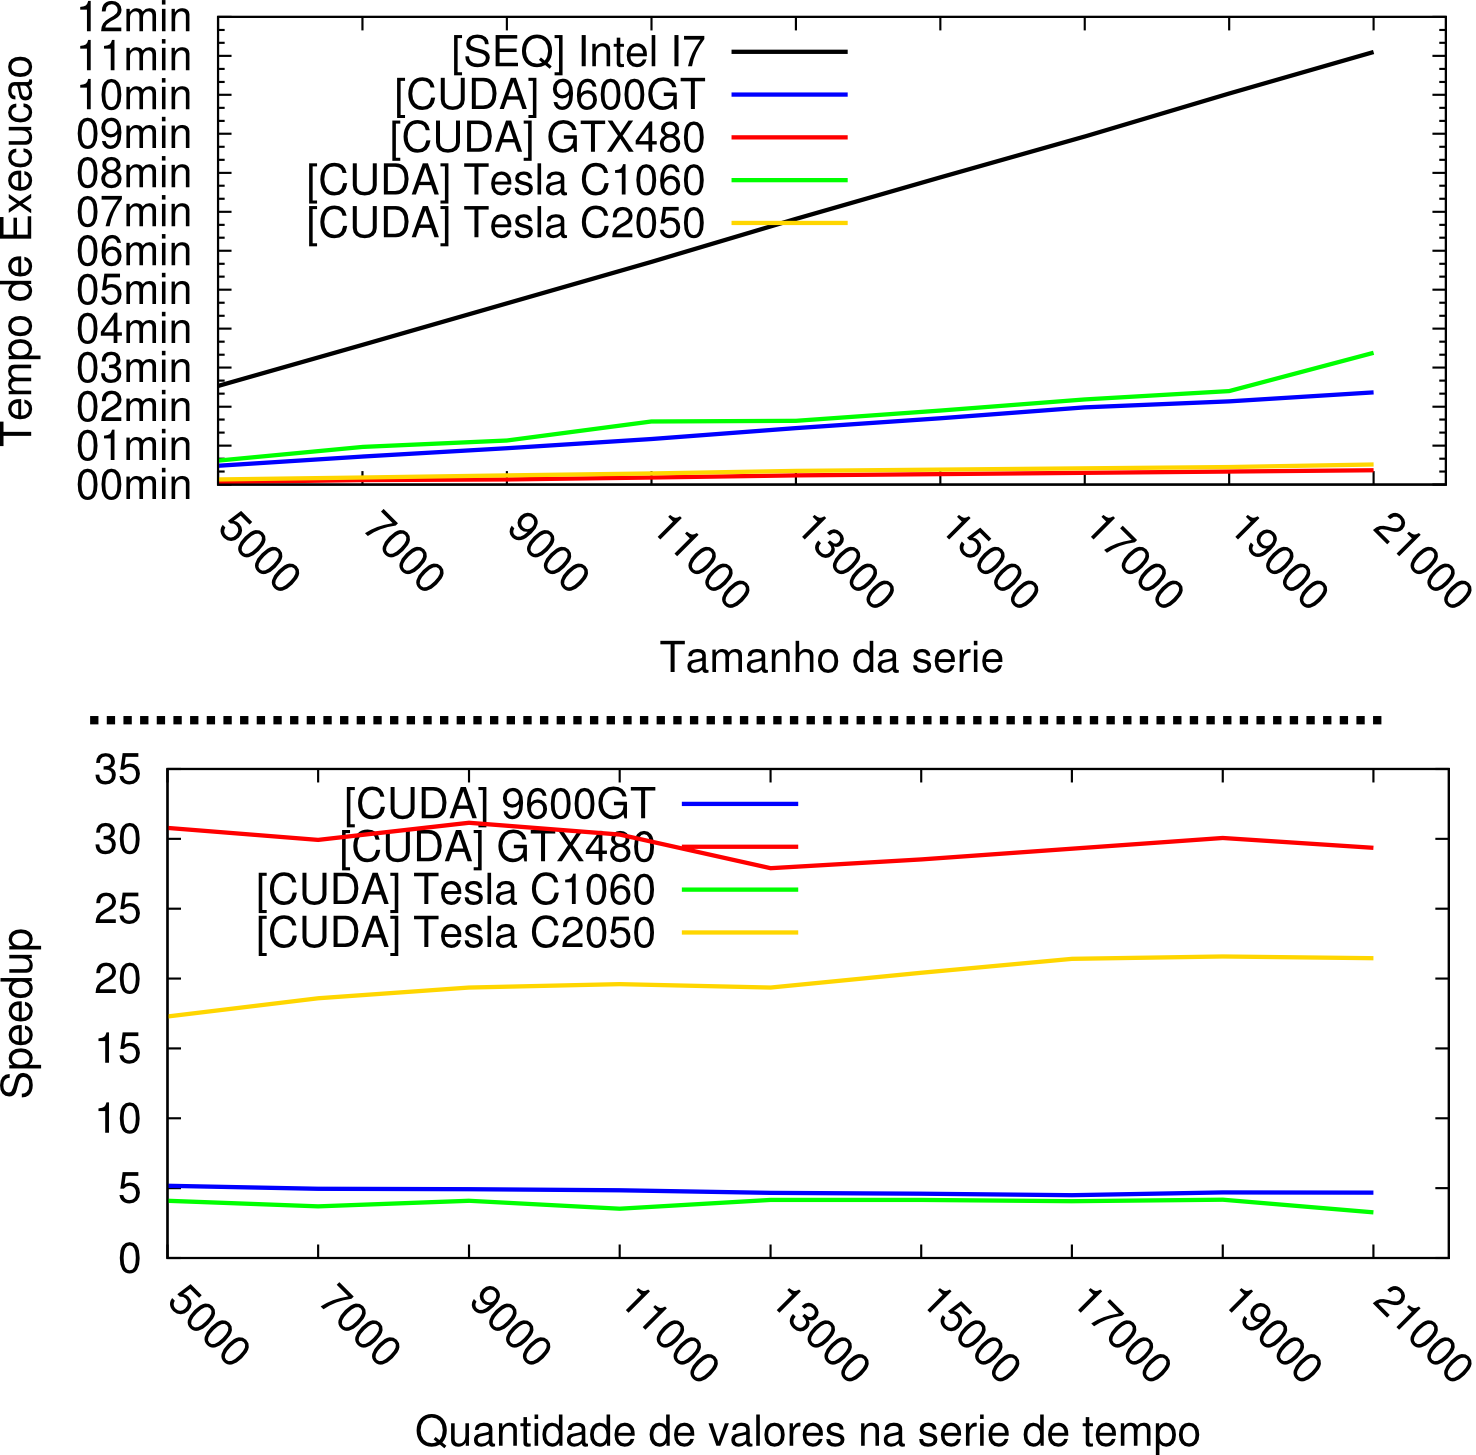
\includegraphics[]{Imagens/graficos_lanczos/lanczos_cuda.png}
\caption{Gráficos do tempo de execução e speedup da implementação em CUDA do algoritmo Filtro de Lanczos}
\label{fig:graficos_lanczos_cuda}
\end{figure}
%%%%%%%%%%%%%%%%%%%%%%%%%%%%%%%%%%%%%%%%%%%%%%%%%%%%%%%%%%

%%%%%%%%%%%%%%%%%%%%%%%%%%%%%%%%%%%%%%%%%%%%%%%%%%%%%%%%%%
% FIGURA
\begin{figure}[H]
\centering
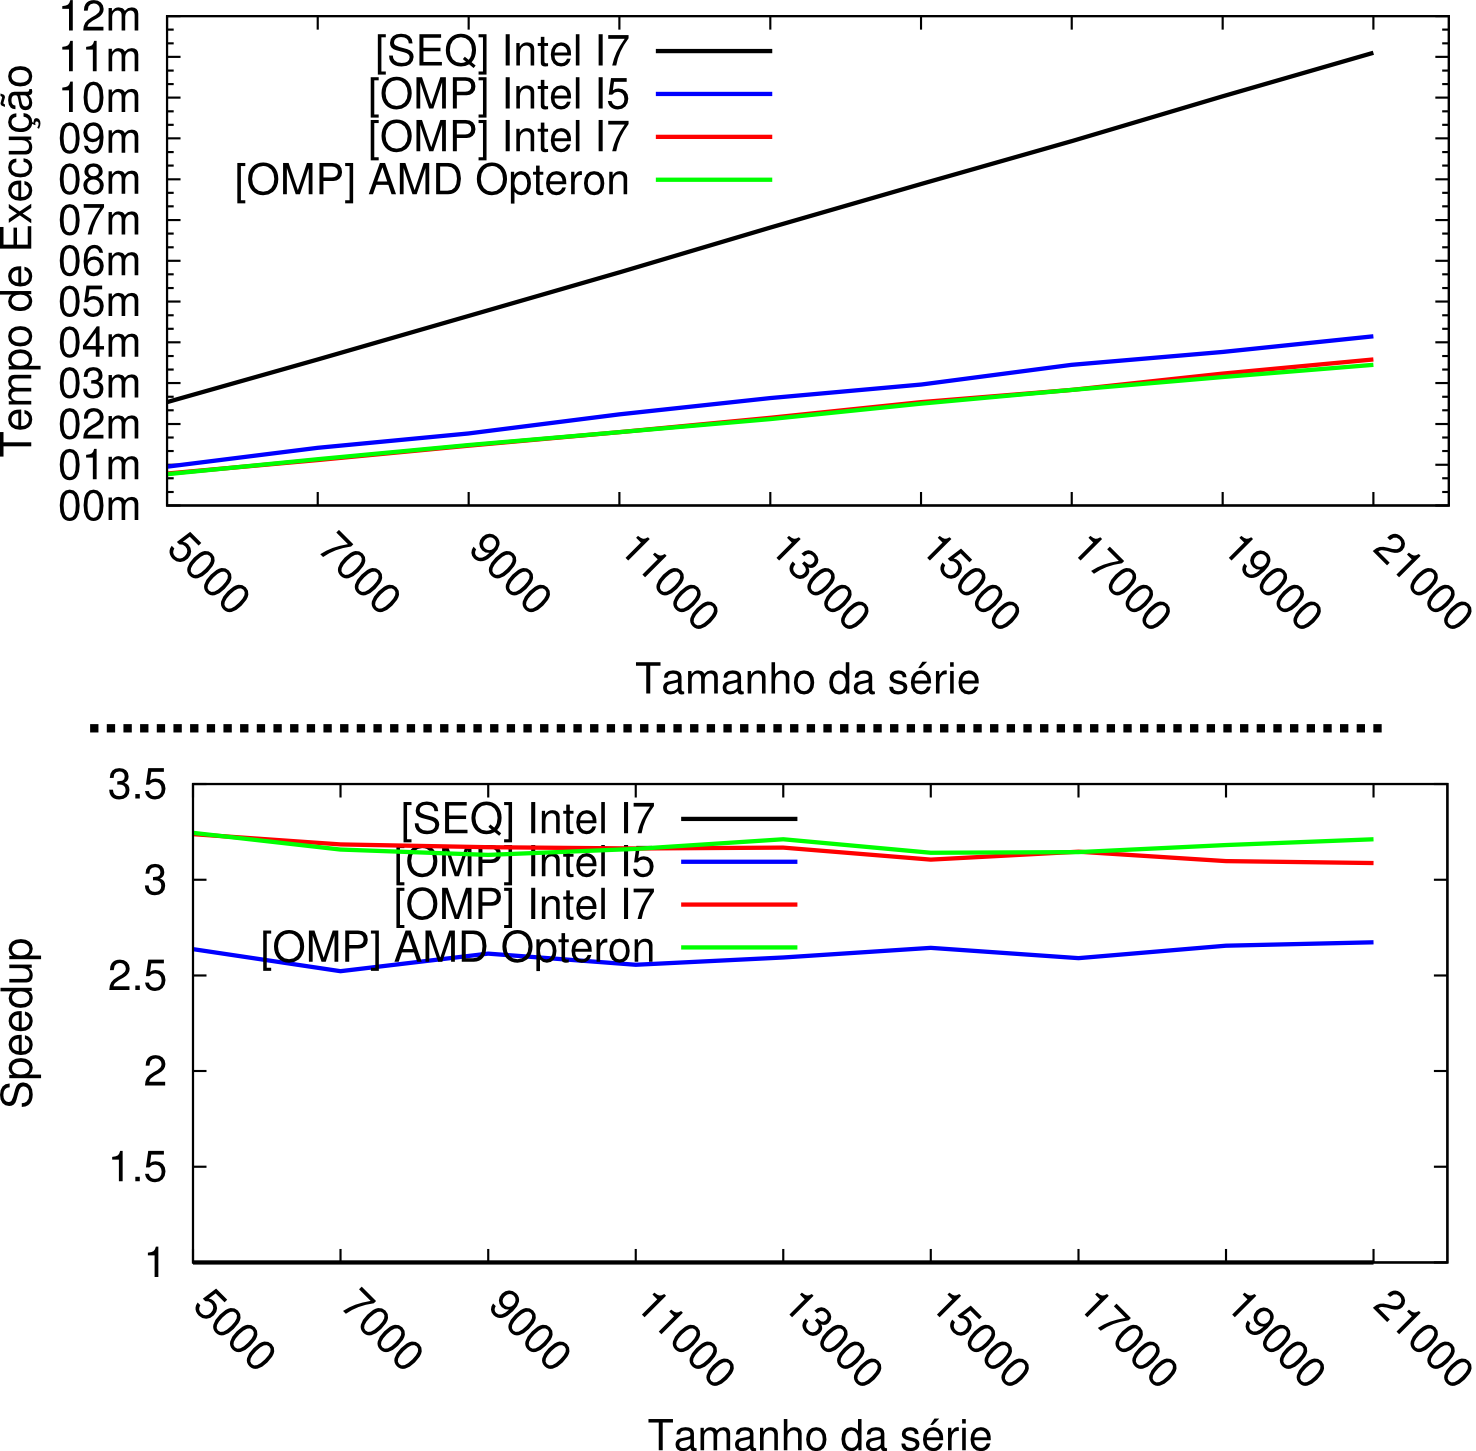
\includegraphics[]{Imagens/graficos_lanczos/lanczos_omp.png}
\caption{Gráficos do tempo de execução e speedup da implementação em OpenMP do algoritmo Filtro de Lanczos}
\label{fig:graficos_lanczos_omp}
\end{figure}
%%%%%%%%%%%%%%%%%%%%%%%%%%%%%%%%%%%%%%%%%%%%%%%%%%%%%%%%%%

\subsection{Resultados obtidos com o algoritmo Teste de Monte Carlo}

Nos testes do algoritmo de Monte Carlo foram usados como dado de entrada uma matriz de 48 por 56 que contém as informações da quantidade de chuva diária na América do Sul entre os anos de 1979 e 1999, totalizando 7665 valores por série, e uma série de chuva de um local na África do mesmo comprimento.
Porém, para questão de comparação, o total de valores usados nos testes foi variado entre 1000 e 5000. Da mesma forma, o número de permutações foi variado entre 1000 e 9000.

%%%%%%%%%%%%%%%%%%%%%%%%%%%%%%%%%%%%%%%%%%%%%%%%%%%%%%%%%%
% FIGURA
\begin{figure}[H]
\centering
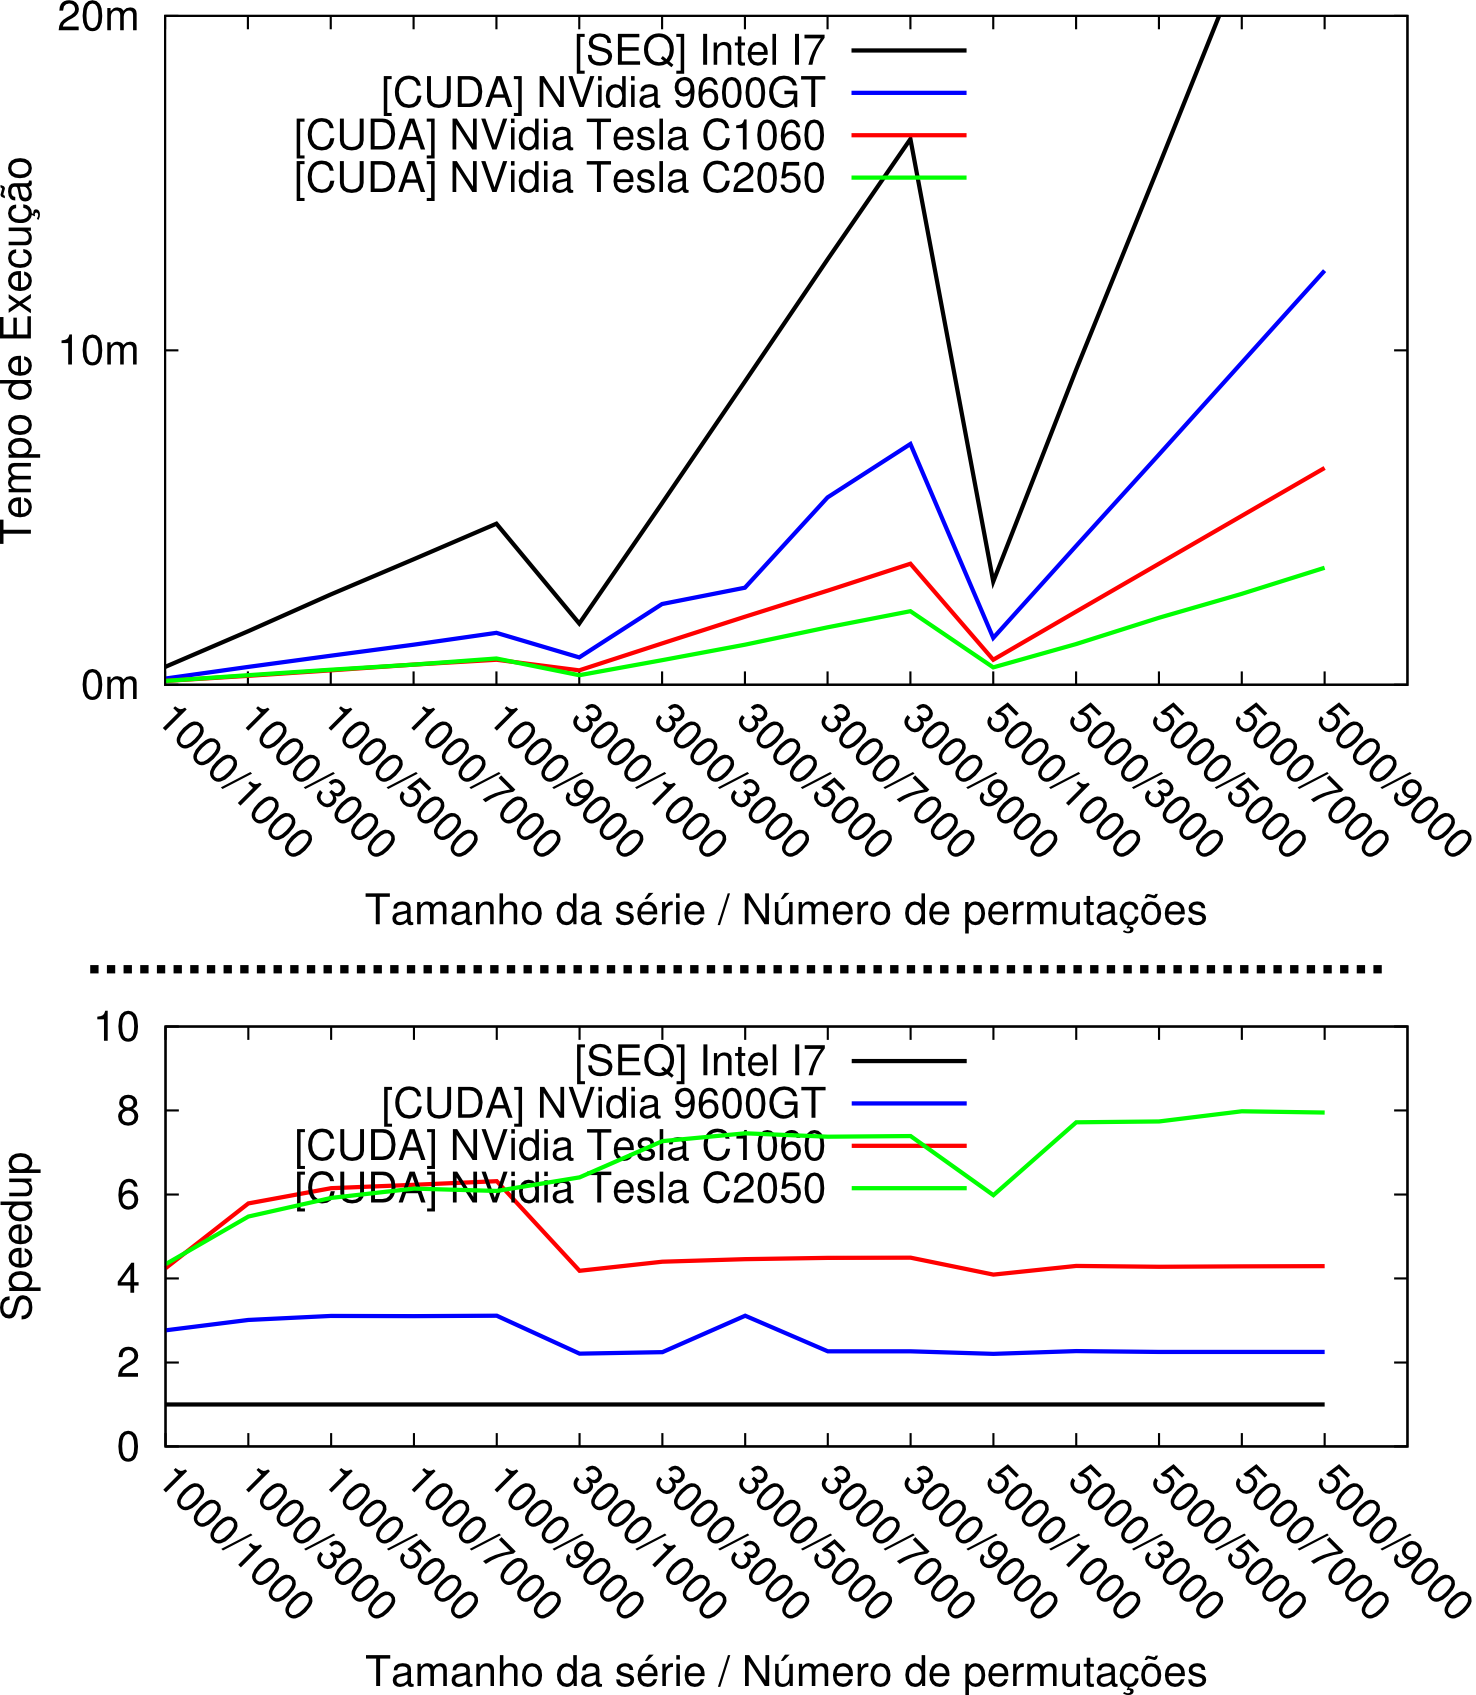
\includegraphics[]{Imagens/graficos_mcarlo/mcarlo_cuda.png}
\caption{Gráficos do tempo de execução e speedup da implementação em CUDA do algoritmo de Monte Carlo}
\label{fig:graficos_mcarlo_cuda}
\end{figure}
%%%%%%%%%%%%%%%%%%%%%%%%%%%%%%%%%%%%%%%%%%%%%%%%%%%%%%%%%%

Nos testes da implementação em OpenMP houve uma grande surpresa, pois o tempo de execução foi incrementado em relação ao tempo de execução sequencial, especialmente ao elevar o número de permutações, como pode ser visto na figura \ref{fig:grafico_mcarlo_omp}. No entanto, nos testes da implementação em CUDA houve uma drástica redução desse tempo, inclusive ao incrementar o número de permutações, como mostrado na figura \ref{fig:graficos_mcarlo_cuda}.

%%%%%%%%%%%%%%%%%%%%%%%%%%%%%%%%%%%%%%%%%%%%%%%%%%%%%%%%%%
% FIGURA
\begin{figure}[H]
\centering
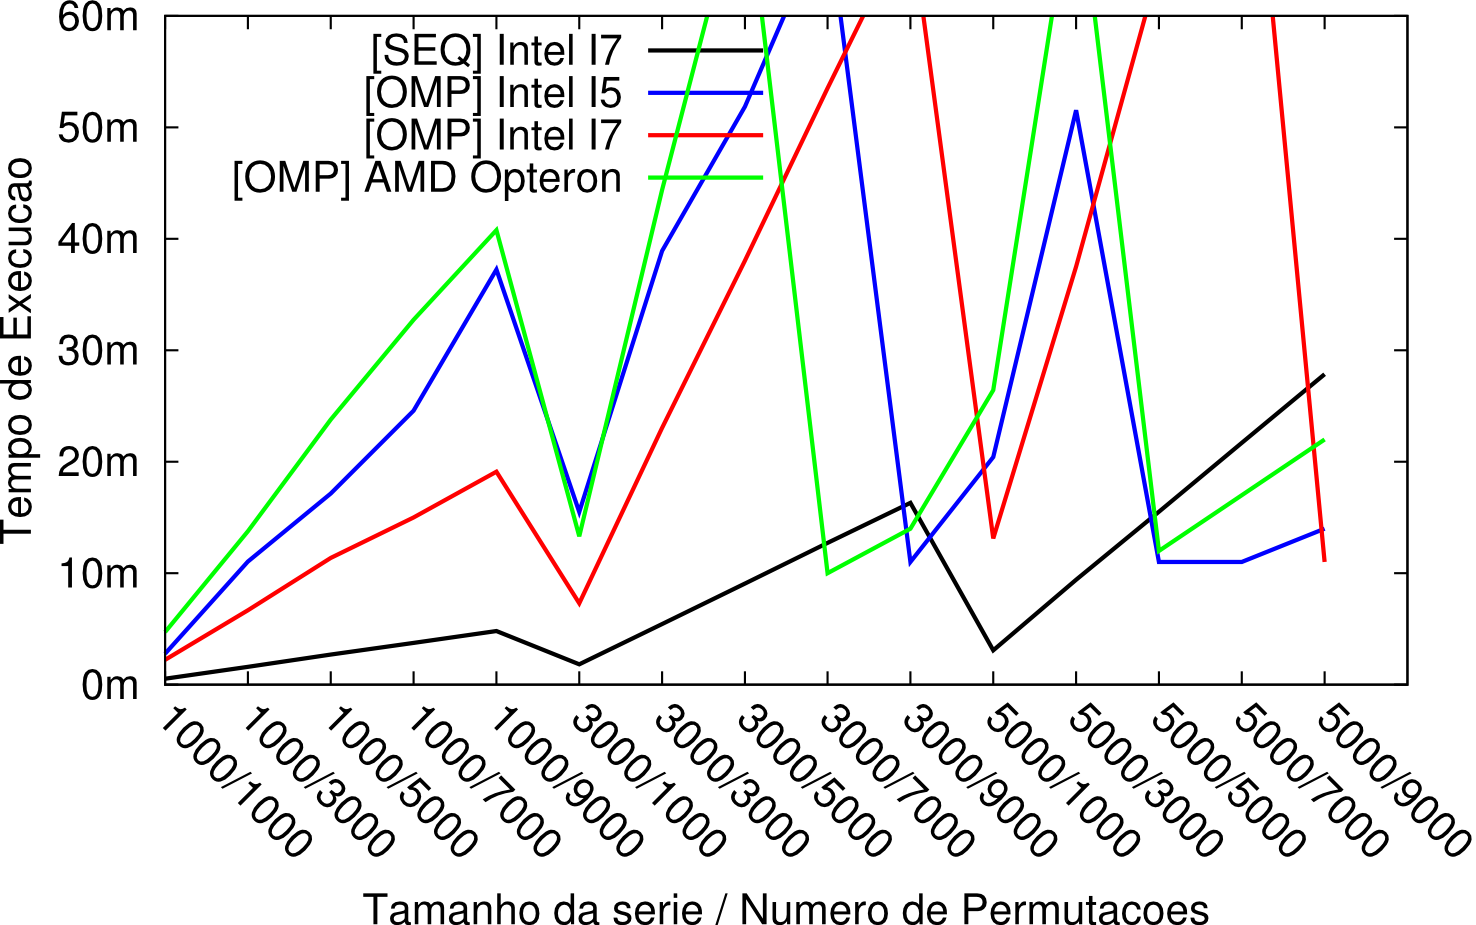
\includegraphics[]{Imagens/graficos_mcarlo/mcarlo_omp.png}
\caption{Gráfico do tempo de execução da implementação em OpenMP do algoritmo Monte Carlo}
\label{fig:grafico_mcarlo_omp}
\end{figure}
%%%%%%%%%%%%%%%%%%%%%%%%%%%%%%%%%%%%%%%%%%%%%%%%%%%%%%%%%%

Uma teoria que explique tais resultados é que pelo fato da implementação em OpenMP prover de apenas uma memória que é compartilhada entre todas as threads, ao se fazer as permutações das séries são realizadas inúmeras requisições simultâneas de escrita na memória que por sua vez não é capaz de responder todas elas imediatamente. Esse atraso faz com que as threads fiquem ociosas durante um longo tempo até que todas as requisições sejam executadas. Ao aumentar o número de permutações, o número de requisições é proporcionalmente incrementado, agravando o problema.

Tal problema não ocorre na implementação em CUDA pois a mesma é executada na GPU, que possui uma arquitetura de memória totalmente diferente a qual provê à cada thread diversos níveis de memória, incluindo uma própria, como descrito na seção 2.3 de \cite{cuda_guide}. Dessa forma as requisições de escrita são distribuídas entre várias memórias independentes reduzindo o congestionamento de requisições.

%%%%%%%%%%%%%%%%%%%%%%%%%%%%%%%%%%%%%%%%%%%%%%%%%%%%%%%%%%
% FIGURA
\begin{figure}[H]
\centering
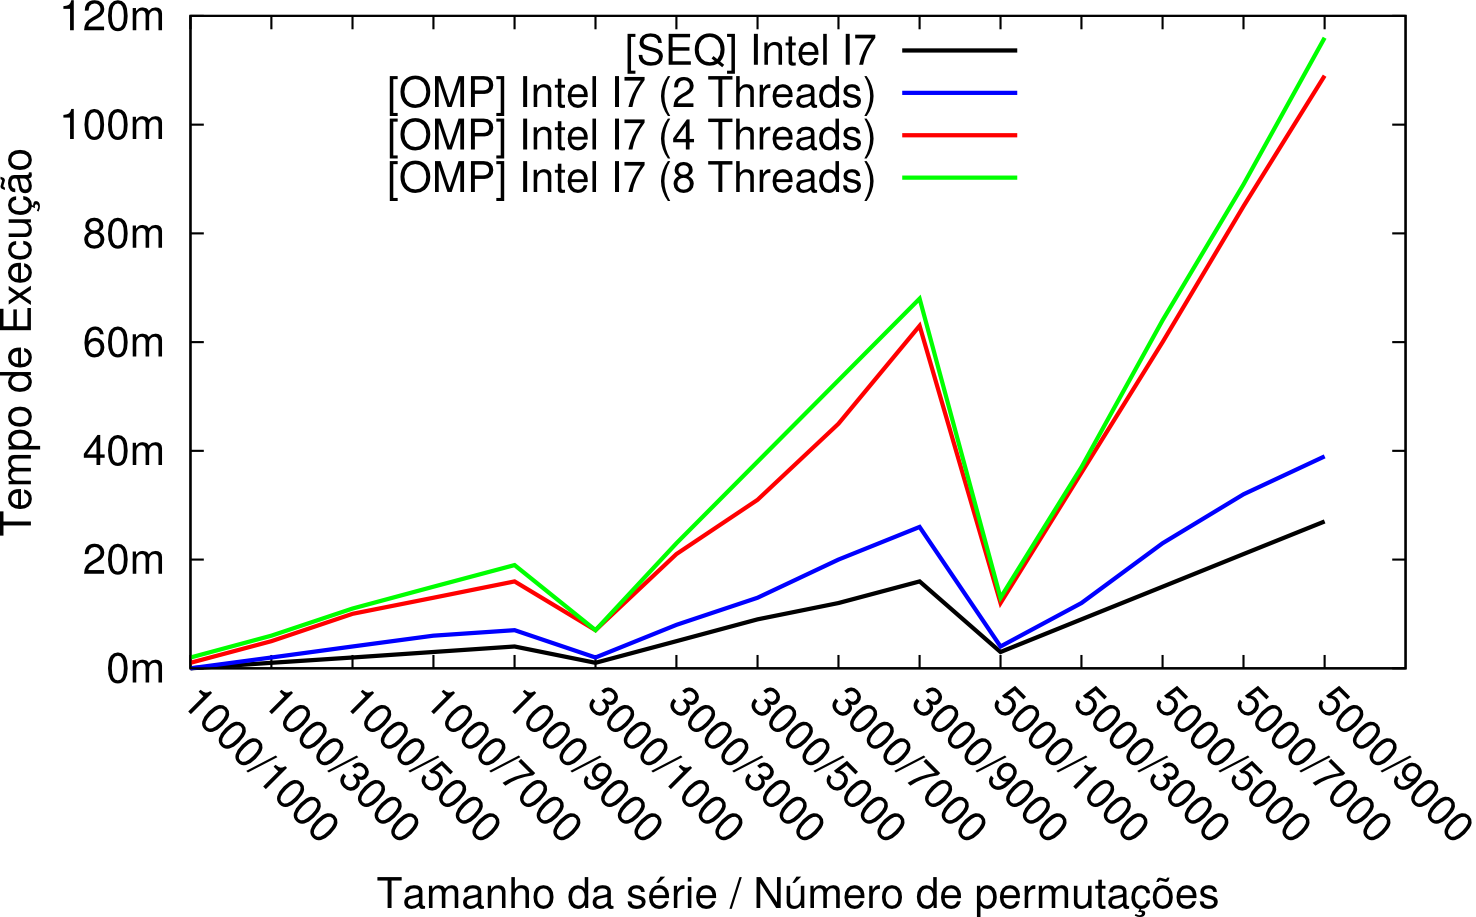
\includegraphics[]{Imagens/graficos_mcarlo/mcarlo_omp-threads.png}
\caption{Gráfico do tempo de execução da implementação em OpenMP do algoritmo Monte Carlo com a variação do número de threads}
\label{fig:grafico_mcarlo_omp_threads}
\end{figure}
%%%%%%%%%%%%%%%%%%%%%%%%%%%%%%%%%%%%%%%%%%%%%%%%%%%%%%%%%%

Para reforçar essa hipótese foram feitos alguns testes reduzindo o número de threads usadas na execução da implementação em OpenMP. Esses resultados estão expostos na figura \ref{fig:grafico_mcarlo_omp_threads}. É perceptível que ao reduzir o número de threads o tempo de execução reduz consideravelmente, pois o total de requisições simultâneas também é reduzida e assim amenizando o problema. Ainda assim os tempos  de execução continuaram maiores do que a implementação sequencial.

Esses resultados são importantes para demonstrar que a arquitetura atual dos computadores não é a ideal para se executar algoritmos paralelos.

\subsection{Tempo gasto para a leitura dos dados usando o modo proposto}

Um fator importante para a análise dos resultados é o tempo gasto para ler e reorganizar os dados do modo proposto na seção \ref{cap:proposta_solucao}, pois essa tarefa agrega um tempo extra ao tempo total de execução que normalmente não existiria. Os gráficos abaixo demonstram a diferença entre o tempo de leitura dos dados usados como entrada para o algoritmo Filtro de Lanczos utilizando o método original e o método proposto, e um comparativo desse tempo de leitura e o tempo total da execução da implementação em CUDA na GPU Tesla C2050.

%%%%%%%%%%%%%%%%%%%%%%%%%%%%%%%%%%%%%%%%%%%%%%%%%%%%%%%%%%
% FIGURA
\begin{figure}[H]
\centering
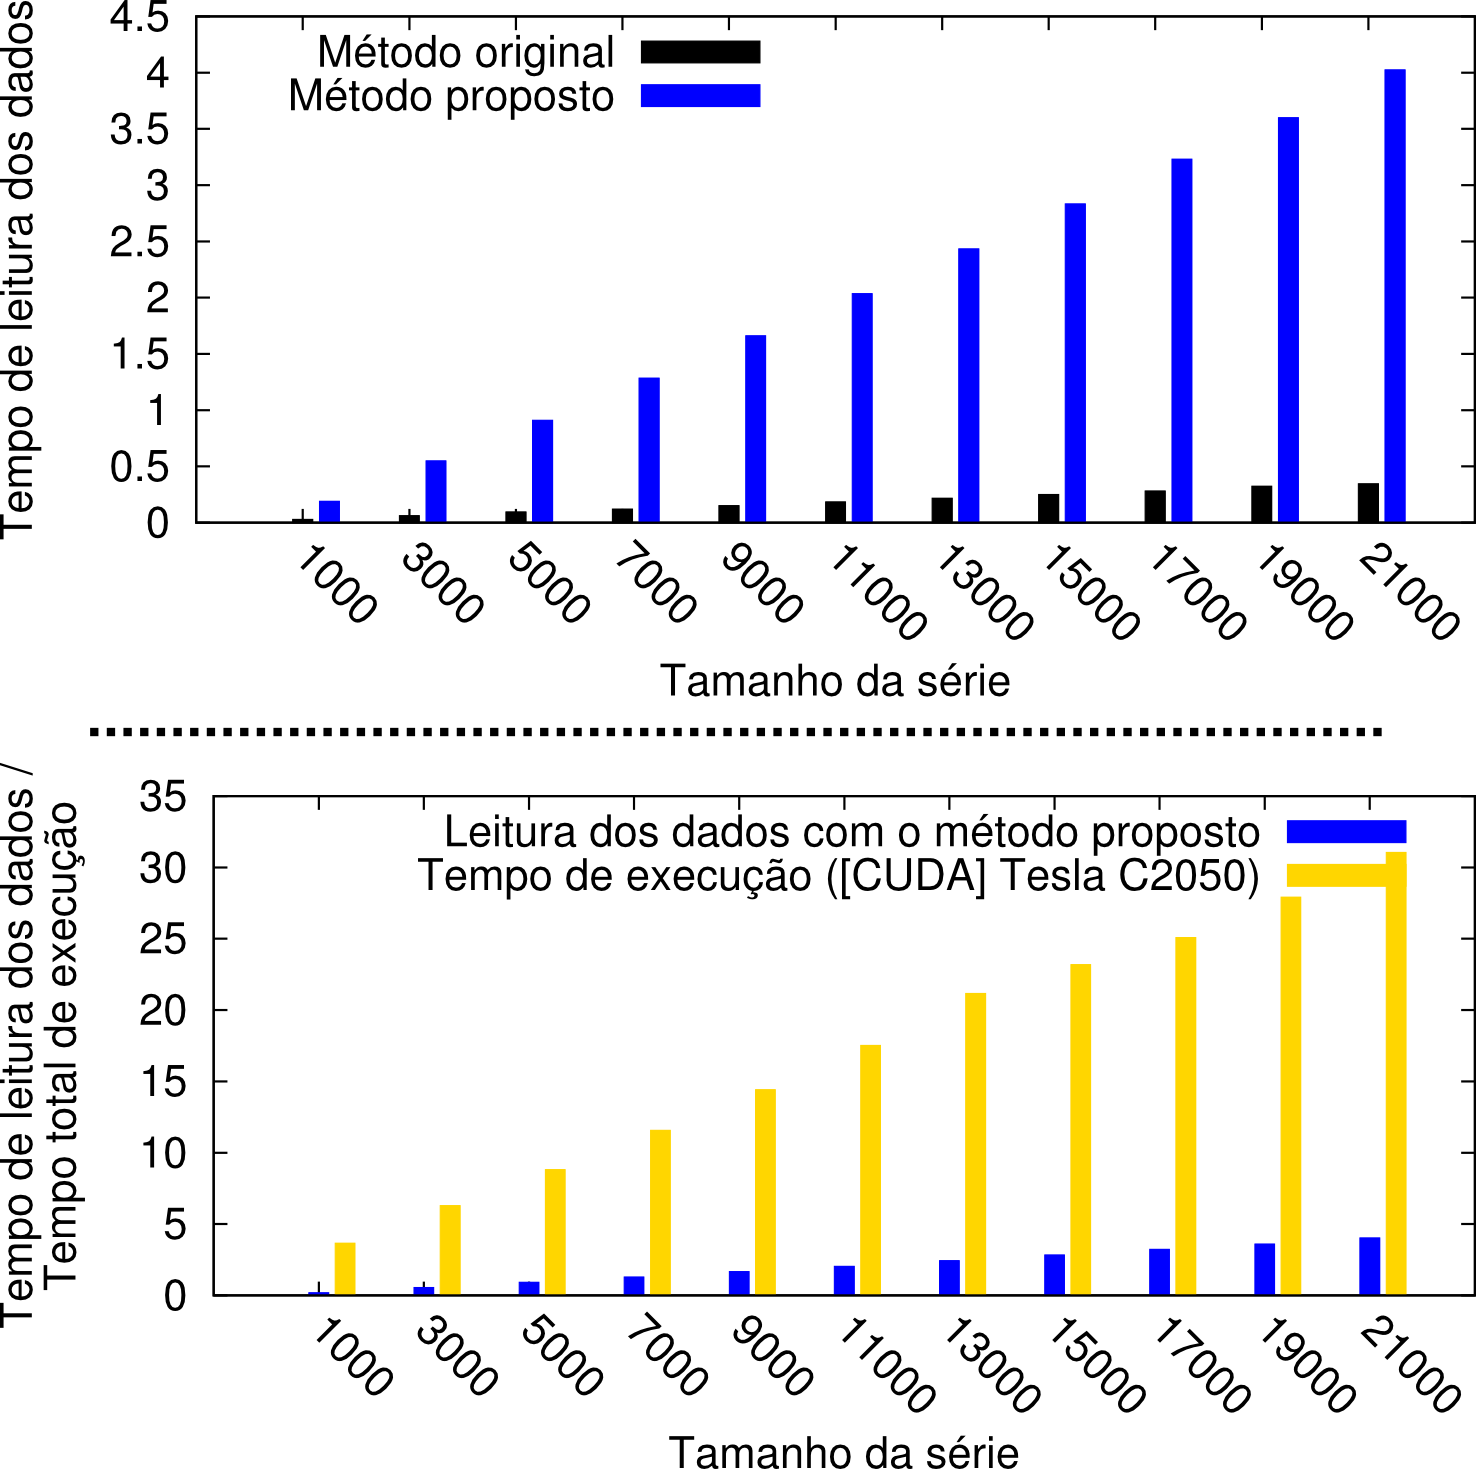
\includegraphics[]{Imagens/grafico_tempo_leitura/lanczos_tempos_leitura.png}
\caption{Gráficos comparativos do tempo de leitura dos dados}
\label{fig:grafico_tempos_leitura}
\end{figure}
%%%%%%%%%%%%%%%%%%%%%%%%%%%%%%%%%%%%%%%%%%%%%%%%%%%%%%%%%%

No exemplo dado, o tempo gasto com a leitura dos dados utilizando o método proposto foi, em média, dez vezes maior que o tempo utilizando o método padrão e representa aproximadamente 10\% do tempo total de execução.

Fica claro que o tempo gasto com a leitura dos dados é maior. Porém, esse tempo extra é necessário para a execução dos algoritmos e não causa um prejuízo tão grande para o tempo total de execução se comparado aos benefícios trazidos.

\section{Análise dos resultados}

Como podemos ver, mesmo com o tempo gasto com a leitura e reorganização dos dados e sem nenhuma otimização tanto no código quanto nos parâmetros de execução do código em CUDA, os tempos de execução da versão CUDA são significantemente menores, apresentando tempos seis vezes menores quando usado uma placa-de-vídeo mais antiga como a GPU 9600GT, e de até 30 vezes com a GPU GTX480 nos testes feitos, comparando-as com a CPU Intel I7, considerada por muitos a mais potente da atualidade.

Muitos dos computadores atuais possuem uma placa-de-vídeo capacitada com a tecnologia CUDA. Porém, na grande maioria das vezes, esse recurso é realmente requisitado apenas para visualização de vídeos e jogos. Sabendo disso os resultados desse trabalho demonstram que esse recurso poderia ser melhor aproveitado para fins acadêmicos.